\newpage
\section{OpenMP}
\label{sec:OpenMP}
The tests related to the OpenMP studies are carried out on the University Workstation.
\noindent
All results were obtained by compiling with the following command (see \texttt{Makefile}) running each version 10 times, and computing the average runtime: \texttt{icpx -O2 -march=native -fopenmp}.
\noindent
I defined the parameters as follows: $RESOLUTION = 10000$ and $ITERATIONS = 100$

\subsection{Parallel For}
In the first approach (\texttt{src/omp1.cpp}), the outer loop over was parallelized by the directive using default static scheduling (\texttt{schedule(static)}).
\begin{lstlisting}[basicstyle=\ttfamily\scriptsize]
    #pragma omp parallel for
    for (int pos = 0; pos < HEIGHT * WIDTH; pos++)
    {
        image[pos] = 0;
        const int row = pos / WIDTH;
        const int col = pos % WIDTH;
        double cRe = col * STEP + MIN_X;
        double cIm = row * STEP + MIN_Y;
        double zRe = 0, zIm = 0;
        for (int i = 1; i <= ITERATIONS; i++)
        {
            double oldRe = zRe;
            zRe = (zRe*zRe - zIm*zIm) + cRe;
            zIm = 2*oldRe*zIm + cIm;

            if(zRe*zRe + zIm*zIm >= 4)
            {
                image[pos] = i;
                break;
            }
        }
    }
\end{lstlisting}

\begin{center}
    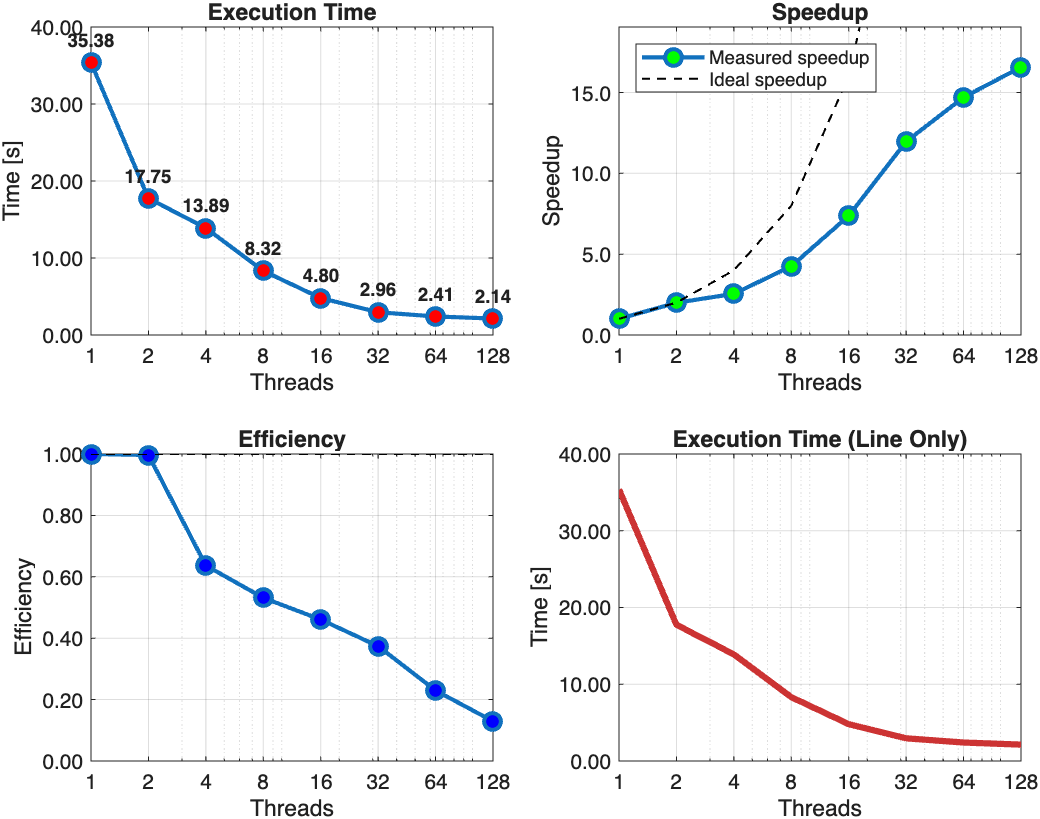
\includegraphics[width=0.85\textwidth]{assets/openmp/omp1.png}
\end{center}

\noindent
Execution times decrease monotonically as the number of threads increases, and the corresponding speedup grows accordingly. As expected, it remains below the theoretical Amdahl limit (considering an almost negligible sequential fraction). Efficiency is high only for the first few threads (1 up to 2), after which load imbalance becomes noticeable.




\subsection{Guided Scheduling}
The following scheduling policy dynamically balances workload distribution. It is essential for handling the computational irregularity of the Mandelbrot set algorithm because different pixels requires different amount of iterations.

\begin{lstlisting}
    #pragma omp parallel for schedule(guided)
    for (int pos = 0; pos < HEIGHT * WIDTH; pos++)
    {
        // ... same content ...
    }
\end{lstlisting}

\begin{center}
    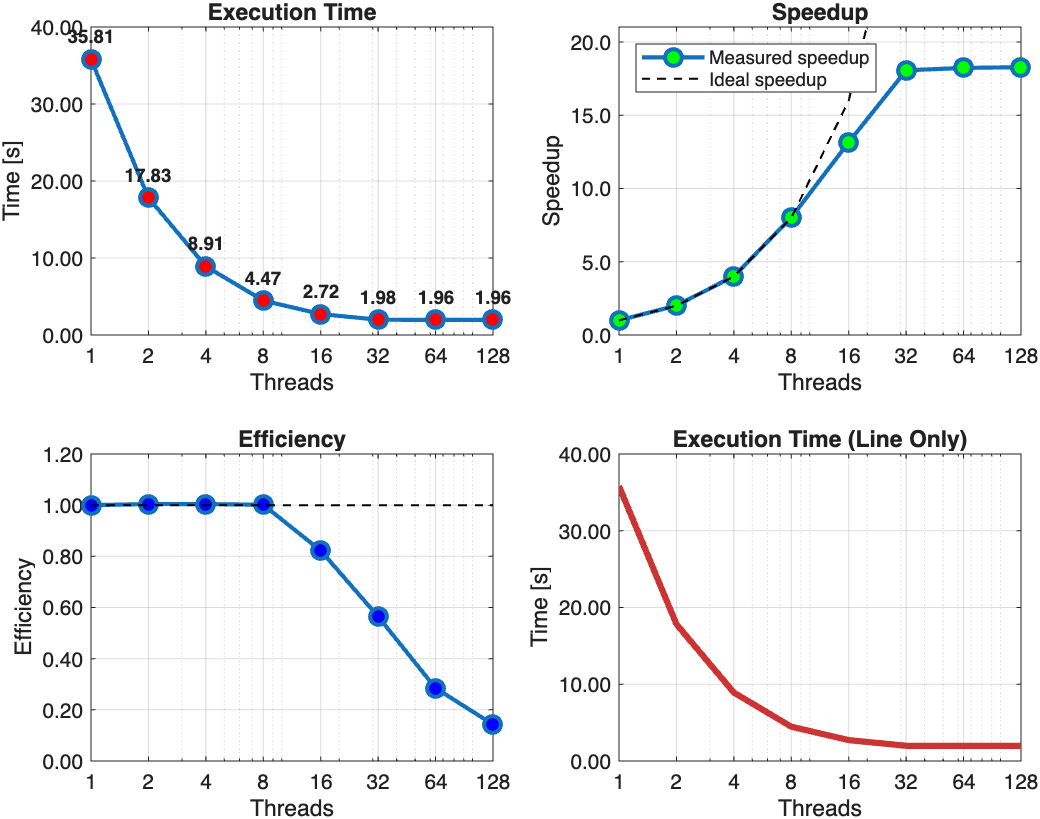
\includegraphics[width=0.9\textwidth]{assets/openmp/omp2.png}
\end{center}

\noindent
Guided scheduling provides clear improvements in both speedup and efficiency. The measured speedup remains close to the theoretical value up to 16 threads (theoretical speedup 16, observed $\approx 13$), corresponding to an efficiency of about 80\%. This demonstrates that guided scheduling effectively mitigates the workload irregularity.


\newpage
\subsection{Guided + SIMD}
Maximum optimization combining multi-thread parallelism with SIMD vectorization.

\begin{lstlisting}
    #pragma omp parallel for simd schedule(guided)
    for (int pos = 0; pos < HEIGHT * WIDTH; pos++)
    {
        // ... same content ...
    }
\end{lstlisting}

\begin{center}
    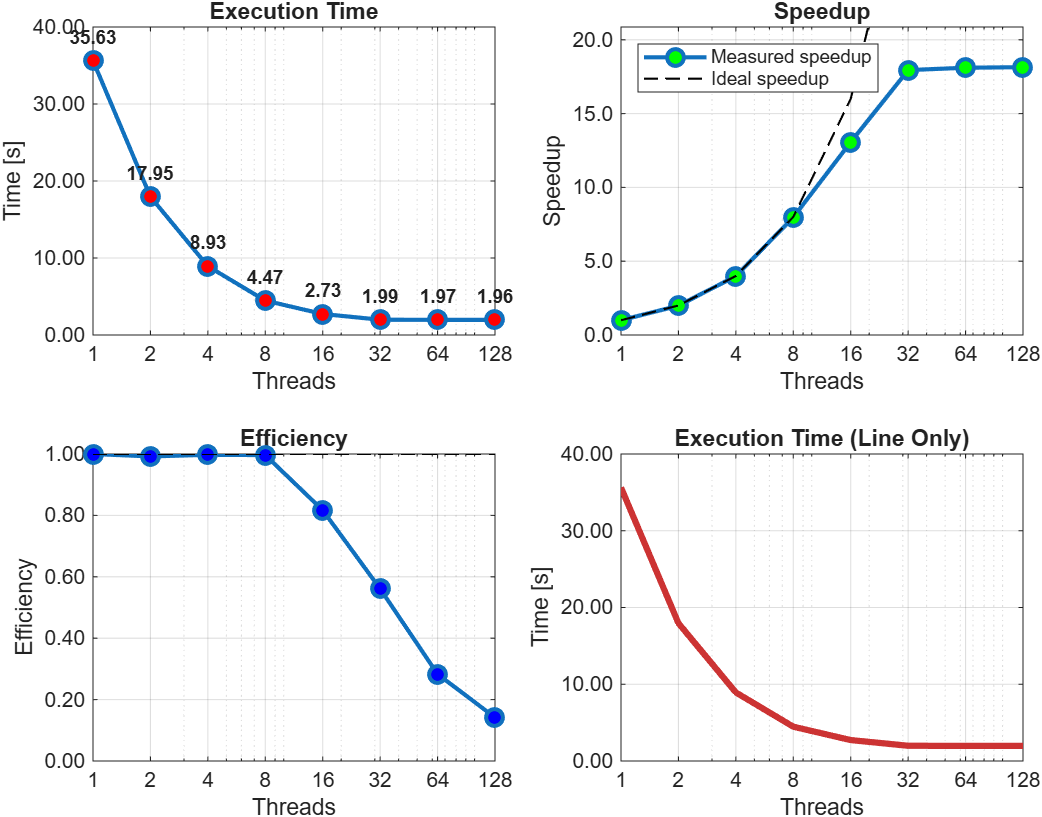
\includegraphics[width=0.9\textwidth]{assets/openmp/omp3.png}
\end{center}

\noindent
The \texttt{simd} clause suggests vectorization, but the Mandelbrot loop includes divergent control flow, which may hinder full vectorization. This is reflected in the results: performance remains essentially unchanged compared to the guided-only version, confirming the difficulty of achieving meaningful SIMD gains in this context.


\subsection{Conclusions}
The static scheduling strategy is not ideal for the Mandelbrot computation because the workload is highly irregular: different pixels require significantly different iteration counts. Guided scheduling, instead, adapts more effectively to this variability and leads to better load balancing.